% Muc 5.5  --  phu trach: Dung (xem report/PHANCONG.md)
% nguon: host/board_classifier.py, host/ecg_layer_host_pc.py
\section{Trình tự thực thi một nhịp}\label{sec:trinhtu}
Để phân loại một nhịp tim, host điều phối bộ tăng tốc theo ba giai đoạn như Hình~\ref{fig:trinhtu}: nạp tín hiệu đầu vào, lặp thực thi từng layer, và đọc kết quả.

\begin{figure}[htbp]\centering
  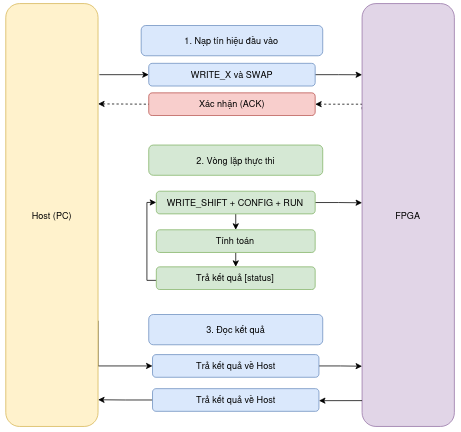
\includegraphics[width=0.7\textwidth]{ch05_giao_thuc_uart/trinh_tu.png}
  \caption{Trình tự lệnh giữa host và FPGA cho một nhịp.}\label{fig:trinhtu}
\end{figure}

\begin{enumerate}
  \item \textbf{Nạp tín hiệu đầu vào.} Host ghi cửa sổ tín hiệu của nhịp vào bộ nhớ ifmap bằng \texttt{WRITE\_X}, sau đó gọi \texttt{SWAP} để dữ liệu này trở thành bank đọc. Mỗi lệnh được FPGA xác nhận bằng \texttt{ACK}.
  \item \textbf{Lặp thực thi từng layer.} Với mỗi layer trong sáu layer của mạng (\texttt{conv0}, \texttt{conv1}, \texttt{conv2}, \texttt{conv3}, \texttt{FC1}, \texttt{FC2}), host gửi \texttt{WRITE\_SHIFT}, \texttt{CONFIG} và \texttt{RUN}. FPGA tính toán trên dữ liệu nằm sẵn trong bộ nhớ trên chip rồi trả về \texttt{RESULT} chứa trạng thái; đầu ra của layer này là đầu vào của layer sau nên không phải đọc về host. Riêng \texttt{FC1} cần thêm đặc trưng RR do host ghi bằng \texttt{WRITE\_X}, và \texttt{FC2} bật cờ \texttt{out\_int32} cùng \texttt{argmax}.
  \item \textbf{Đọc kết quả.} Host gửi \texttt{READ\_FMAP} để nhận logit và nhãn dự đoán của lớp đầu ra.
\end{enumerate}

Tham số của mô hình (trọng số, bias) có thể được cấp theo hai cách do phần mềm host lựa chọn:
\begin{itemize}
  \item \textbf{Gửi lại theo từng layer:} trước mỗi layer, host ghi trọng số và bias của layer đó vào bộ nhớ.
  \item \textbf{Nạp một lần (\texttt{--resident}):} host ghi toàn bộ trọng số và bias của mạng vào hai bank trọng số và bộ nhớ bias ngay từ đầu. Mỗi layer sau đó dùng \texttt{w\_base} và \texttt{b\_base} trong \texttt{CONFIG} để trỏ đến vùng tham số của mình, và host chỉ dùng \texttt{SWAP} đổi bank trọng số đọc giữa các nhóm layer. Cách này loại bỏ việc gửi lại tham số ở mỗi nhịp.
\end{itemize}
